% !TeX program = xelatex
\documentclass[a4paper,10pt]{article}

% ============================================================================
% សន្លឹកកិច្ចការសិស្ស ស-ខ្មៅ (Student Guided-Inquiry Worksheet - Grade 8 ALG57)
% បរិបទ៖ ថ្នាក់រៀនគ្មានស្លាយ LCD – ៤.១ និង ៤.២ ការដាក់ជាផលគុណកត្តាដោយកត្តារួម និងសមភាពសំខាន់ៗ (២ ទំព័រ A4)
% ============================================================================
\usepackage[a4paper, left=0.90cm, right=0.90cm, top=0.75cm, bottom=0.85cm, footskip=0.45cm]{geometry}
\usepackage{amsmath, amssymb}
\usepackage{unicode-math}
\usepackage{fontspec}
\usepackage{array, colortbl}
\usepackage[table]{xcolor}
\usepackage{enumitem}
\usepackage{pifont}
\usepackage{fancyhdr}
\usepackage{lastpage}
\usepackage{tikz}
\usepackage[most]{tcolorbox}
\usetikzlibrary{calc, arrows.meta, positioning, babel}

\makeatletter
\let\@expl@@@mark@update@singlecol@structures@@\relax
\makeatother

\providecommand{\NGSFindFonts}{%
  \IfFileExists{C:/Windows/Fonts/cambria.ttc}{%
    \def\NGSSysPath{C:/Windows/Fonts/}%
    \def\NGSUserPath{C:/Users/KIT/AppData/Local/Microsoft/Windows/Fonts/}%
  }{%
    \IfFileExists{./fonts/KhmerOSsiemreap.ttf}{\def\NGSSysPath{./fonts/}\def\NGSUserPath{./fonts/}}{%
    \IfFileExists{../fonts/KhmerOSsiemreap.ttf}{\def\NGSSysPath{../fonts/}\def\NGSUserPath{../fonts/}}{%
    \IfFileExists{../../fonts/KhmerOSsiemreap.ttf}{\def\NGSSysPath{../../fonts/}\def\NGSUserPath{../../fonts/}}{%
    \IfFileExists{../../../fonts/KhmerOSsiemreap.ttf}{\def\NGSSysPath{../../../fonts/}\def\NGSUserPath{../../../fonts/}}{%
    \IfFileExists{../../../../fonts/KhmerOSsiemreap.ttf}{\def\NGSSysPath{../../../../fonts/}\def\NGSUserPath{../../../../fonts/}}{%
    \IfFileExists{../../../../../fonts/KhmerOSsiemreap.ttf}{\def\NGSSysPath{../../../../../fonts/}\def\NGSUserPath{../../../../../fonts/}}{%
    \IfFileExists{../../../../../../fonts/KhmerOSsiemreap.ttf}{\def\NGSSysPath{../../../../../../fonts/}\def\NGSUserPath{../../../../../../fonts/}}{%
      \def\NGSSysPath{../../../../../../../fonts/}\def\NGSUserPath{../../../../../../../fonts/}%
    }}}}}}}%
  }%
}
\NGSFindFonts

\setmathfont[Path={\NGSSysPath}, FontIndex=1, Scale=1.02]{cambria.ttc}
\defaultfontfeatures{Ligatures=TeX}

\setmainfont[
  Path={\NGSUserPath},
  Extension=.ttf,
  Script=Khmer,
  BoldFont={KhmerOSsiemreap},
  BoldFeatures={FakeBold=1.8},
  ItalicFont={KhmerOSsiemreap},
  ItalicFeatures={FakeSlant=0.25},
  BoldItalicFont={KhmerOSsiemreap},
  BoldItalicFeatures={FakeBold=1.8, FakeSlant=0.25}
]{KhmerOSsiemreap}

\newfontfamily\muol[Path={\NGSUserPath}, Extension=.ttf, Script=Khmer]{KhmerOSmuollight}
\newfontfamily\TimesEn[Path={\NGSSysPath}, Extension=.ttf, BoldFont={timesbd}, ItalicFont={timesi}, BoldItalicFont={timesbi}]{times}

\XeTeXlinebreaklocale "km"
\XeTeXlinebreakskip = 0pt plus 1pt minus 0.1pt

\definecolor{panelgray}{gray}{0.94}
\definecolor{headgray}{gray}{0.86}

\pagestyle{fancy}
\fancyhf{}
\renewcommand{\headrulewidth}{0pt}
\fancyfoot[L]{\fontsize{8pt}{10pt}\selectfont អនុវិទ្យាល័យព្រះក្រសាំង \en{|} គណិតវិទ្យា ថ្នាក់ទី៨ \en{|} មេរៀនទី៥ (៤.១--៤.២ ការដាក់ជាផលគុណកត្តាដោយកត្តារួម និងសមភាពសំខាន់ៗ)}
\fancyfoot[R]{\fontsize{8.2pt}{10pt}\selectfont ទំព័រ \en{\thepage\ / \pageref{LastPage}}}

\setlength{\parindent}{0pt}
\setlength{\parskip}{0pt}
\setlength{\tabcolsep}{4pt}

\newcommand{\en}[1]{{\TimesEn #1}}
\newcommand{\enbf}[1]{{\TimesEn\textbf{#1}}}
\newcommand{\unit}[1]{\,\text{\en{#1}}}
\newcommand{\cnum}[1]{{\fontsize{10pt}{12pt}\selectfont\ding{\numexpr171+#1\relax}}}
\newcommand{\chk}{\tikz[baseline=-0.15ex]\draw[black, line width=0.8pt] (0,0) rectangle (0.25cm,0.25cm);}
\newcommand{\dotline}[1]{\makebox[#1]{\dotfill}}

\newcolumntype{L}[1]{>{\raggedright\arraybackslash}p{#1}}
\newcolumntype{C}[1]{>{\centering\arraybackslash}p{#1}}

\newcommand{\secbar}[2]{%
  \vspace{5pt}
  \noindent\colorbox{headgray}{\parbox{\dimexpr\linewidth-2\fboxsep\relax}{%
    \vspace{1.8pt}{\muol\fontsize{9.5pt}{13.5pt}\selectfont #1}\hfill{\fontsize{8.5pt}{12pt}\selectfont\textbf{#2}}\vspace{1.8pt}%
  }}\par\vspace{5pt}
}

\begin{document}
\fontsize{9.5pt}{14.2pt}\selectfont

% ============================================================================
% ទំព័រទី១៖ ក្បាលសន្លឹកកិច្ចការ + E1 + E2 + E3
% ============================================================================
\begin{tcolorbox}[enhanced, sharp corners, colback=white, colframe=black, boxrule=1.0pt, top=4pt, bottom=4pt, left=6pt, right=6pt]
  \begin{center}
    {\muol\fontsize{10.5pt}{15pt}\selectfont សន្លឹកកិច្ចការសិស្ស — មេរៀនទី៥៖ កន្សោមពីជគណិត \enbf{(}៤.១--៤.២ ការដាក់ជាផលគុណកត្តា\enbf{)}}\\[2pt]
    {\footnotesize សៀវភៅសិក្សាគោលថ្នាក់ទី៨ ទំព័រ ៦៨--៧០ \en{|} កត្តារួមជាកញ្ចប់ និងមែកធាងសម្រេចចិត្តតាមសមភាពសំខាន់ៗ (គ្មានស្លាយ \en{LCD})}
  \end{center}
  \vspace{2pt}
  \hrule height 0.5pt
  \vspace{4pt}
  ឈ្មោះសិស្ស៖ \dotline{5.3cm} ថ្នាក់៖ \dotline{2.0cm} ដៃគូទី៖ \dotline{2.0cm} កាលបរិច្ឆេទ៖ \dotline{3.3cm}
\end{tcolorbox}

% -------------------- ផ្នែកទី១៖ E1 ENGAGE --------------------
\secbar{ផ្នែកទី១ ៖ បេសកកម្មភ្ជាប់បញ្ហា \enbf{(E1 — Engage)} — ដំណើរបញ្ច្រាសពីផលបូកទៅផលគុណកត្តា}{\en{3} នាទី (ទស្សន៍ទាយមុនរៀន)}

\begin{tcolorbox}[enhanced, sharp corners, colback=panelgray, colframe=black, boxrule=0.8pt, top=3.5pt, bottom=3.5pt, left=6pt, right=6pt]
  \begin{minipage}[c]{12.3cm}
    ១) រងបន្លែ ៣ ជាប់គ្នាមានក្រឡាផ្ទៃសរុប $3x + 3y + 3z = 3(\dotline{2.5cm})$ ។\\[2pt]
    ២) \textbf{ទស្សន៍ទាយមុនរៀន៖} តើកន្សោម $(3x+2y)(x+1) - y(x+1)$ ស្មើនឹងផលគុណកត្តាមួយណា?\\[1.5pt]
    \hspace*{0.3cm}\chk\ $(x+1)(3x+2y)$ \qquad
    \chk\ $(x+1)(3x+y)$ \qquad
    \chk\ $(x+1)^2(3x+y)$
  \end{minipage}\hfill
  \begin{minipage}[c]{5.9cm}
    \centering
    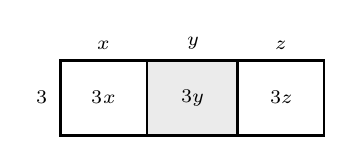
\begin{tikzpicture}[every node/.style={font=\scriptsize}]
      \draw[line width=0.85pt, fill=white] (0,0) rectangle (1.1,0.95);
      \draw[line width=0.85pt, fill=gray!16] (1.1,0) rectangle (2.25,0.95);
      \draw[line width=0.85pt, fill=white] (2.25,0) rectangle (3.35,0.95);
      \node at (0.55,0.48) {$3x$};
      \node at (1.68,0.48) {$3y$};
      \node at (2.80,0.48) {$3z$};
      \node[left=1pt] at (0,0.48) {$3$};
      \node[above=0.5pt] at (0.55,0.95) {$x$};
      \node[above=0.5pt] at (1.68,0.95) {$y$};
      \node[above=0.5pt] at (2.80,0.95) {$z$};
    \end{tikzpicture}
  \end{minipage}
\end{tcolorbox}

% -------------------- ផ្នែកទី២៖ E2 EXPLORE --------------------
\secbar{ផ្នែកទី២ ៖ រុករកកត្តារួម និងការដាក់កត្តាតាមសមភាពសំខាន់ៗ \enbf{(E2 — Explore)}}{\en{11} នាទី (ពិភាក្សាដៃគូ)}

\textbf{ក. សកម្មភាពទី១ (រុករក ៤.១ កត្តារួមជាឯកធា និងជាកញ្ចប់វង់ក្រចក ទំ.៦៨--៦៩)៖}
\begin{enumerate}[label=\arabic*., leftmargin=0.55cm, itemsep=4.5pt, topsep=2pt]
  \item \textbf{កត្តារួមជាចំនួន ឬឯកធា (ឧទាហរណ៍ទី១ ទំ.៦៨)៖} $3x + 3y + 3z = \dotline{0.9cm}(x + y + z)$ \;;\; $5a^2 - 15ab = 5a(\dotline{2.2cm})$ ។
  \item \textbf{កត្តារួមជាកញ្ចប់ទ្វេធា (ឧទាហរណ៍ទី២ ទំ.៦៨)៖} គូសបន្ទាត់ក្រោមកញ្ចប់ដូចគ្នា រួចដាក់ជាកត្តារួម៖\\
  $x\underline{(2b - 3)} + y\underline{(2b - 3)} = (2b - 3)(\dotline{2.2cm})$ ។
  \item \textbf{លំហាត់គំរូ (ទំ.៦៩)៖} $(3x + 2y)\underline{(x + 1)} - y\underline{(x + 1)} = (x + 1)(3x + 2y - \dotline{0.9cm}) = (x + 1)(\dotline{2.2cm})$ ។
  \item \textbf{បង្កើតកញ្ចប់កត្តារួម (១១ខ ទំ.៧៣)៖} $(3a^2 - 12a) - 5(a - 4) = 3a(\dotline{1.8cm}) - 5(a - 4) = (\dotline{1.8cm})(\dotline{2.0cm})$ ។
\end{enumerate}

\vspace{5pt}
\textbf{ខ. សកម្មភាពទី២ (រុករក ៤.២ ការដាក់កត្តាតាមសមភាពសំខាន់ៗ $(a\pm b)^2$, $a^2-b^2$ និង $a^3\pm b^3$ ទំ.៦៩--៧០)៖}
\begin{enumerate}[label=\arabic*., leftmargin=0.55cm, itemsep=4.5pt, topsep=2pt]
  \item \textbf{ផ្ទៀងផ្ទាត់ត្រីធាការេទ្វេធា (ឧទាហរណ៍ ក, ខ ទំ.៦៩)៖}\\
  $\bullet$ $4a^2 + 12a + 9 = (2a)^2 + 2(2a)(3) + 3^2 = (\dotline{2.0cm})^2 = (\dotline{2.0cm})(\dotline{2.0cm})$ ។\\
  $\bullet$ $\dfrac{x^2}{4} - 4x + 16 = \left(\dfrac{x}{2}\right)^2 - 2\left(\dfrac{x}{2}\right)(4) + 4^2 = \left(\dotline{2.0cm}\right)^2$ \;;\; \textbf{អន្ទាក់៖} ចុះ $x^2 + 6x + 16$ អាចដាក់ជា $(x+4)^2$ ដែរឬទេ? \chk\ បាន \; \chk\ មិនបាន (ព្រោះ $2(x)(4) = \dotline{1.1cm} \ne 6x$) ។
  \item \textbf{ផលដកពីរការេ និងផលបូក-ដកពីរគូប (ទំ.៧០ និងទំ.៧៤)៖}\\
  $\bullet$ ការេ៖ $9x^2 - 4 = (3x)^2 - 2^2 = (\dotline{1.8cm})(\dotline{1.8cm})$ \;;\; គូប៖ $8x^3 + y^3 = (2x + y)(\dotline{3.5cm})$ \\
  $\bullet$ ផលដកពីរគូប៖ $27y^3 - 64 = (3y)^3 - 4^3 = (3y - 4)(\dotline{4.0cm})$ ។
\end{enumerate}

\vspace{5pt}
% -------------------- ផ្នែកទី៣៖ E3 EXPLAIN --------------------
\secbar{ផ្នែកទី៣ ៖ មែកធាងវិធានដាក់ជាផលគុណកត្តា \enbf{(E3 — Explain)}}{\en{6} នាទី (កត់ត្រាខ្លឹមសារគោល)}

\begin{tcolorbox}[enhanced, sharp corners, colback=white, colframe=black, boxrule=0.85pt, top=5.5pt, bottom=5.5pt, left=6pt, right=6pt]
  \cnum{1} \textbf{ជំហានទី១ (ចាប់កត្តារួមជាមុនជានិច្ច)៖} $ka + kb = \dotline{3.2cm}$ \quad (ដែល $k$ អាចជាចំនួន ឯកធា ឬកញ្ចប់វង់ក្រចក) ។\\[5pt]
  \cnum{2} \textbf{ករណី ២ តួ (ផលដកពីរការេ)៖} $a^2 - b^2 = \dotline{3.8cm}$ \quad \textit{(ខណៈ $a^2+b^2$ មិនអាចដាក់ជាកត្តាដឺក្រេទី១ ទេ!)} ។\\[5pt]
  \cnum{3} \textbf{ករណី ២ តួ (ផលបូកពីរគូប)៖} $a^3 + b^3 = \dotline{5.2cm}$ \quad (ទ្វេធាបូក $\to$ ត្រីធាដកតួកណ្ដាល $-ab$) ។\\[5pt]
  \cnum{4} \textbf{ករណី ២ តួ (ផលដកពីរគូប)៖} $a^3 - b^3 = \dotline{5.2cm}$ \quad (ទ្វេធាដក $\to$ ត្រីធាបូកទាំងអស់ $+ab$) ។\\[5pt]
  \cnum{5} \textbf{ករណី ៣ តួ (ត្រីធាការេទ្វេធា)៖} ផ្ទៀងតួកណ្ដាល $\pm 2ab$ រួចដាក់៖ $a^2 \pm 2ab + b^2 = \dotline{3.5cm}$ ។\par\vspace{5.5pt}
  {\centering
  
\begin{tikzpicture}
    \node[draw=black, line width=0.8pt, fill=panelgray, inner xsep=10pt, inner ysep=5pt, font=\footnotesize] {គន្លឹះមាស៖ កុំទាន់ប្រញាប់ថាដាក់កត្តាមិនកើត! ចូរចាប់ \textbf{កត្តារួម (\enbf{GCF})} ចេញសិន នោះសមភាពសំខាន់ៗនឹងលេចឡើងភ្លាម!};
  \end{tikzpicture}\par}
\end{tcolorbox}

\newpage
% ============================================================================
% ទំព័រទី២៖ E4 (លំហាត់គំរូ ទំ.៦៩-៧០, ៧៤) + E5 (ប្រតិបត្តិ + Exit Check) + កិច្ចការផ្ទះ
% ============================================================================

% -------------------- ផ្នែកទី៤៖ E4 ELABORATE --------------------
\secbar{ផ្នែកទី៤ ៖ អនុវត្តលំហាត់គំរូ និងករណីពីរដំណាក់កាល \enbf{(E4 — Elaborate)}}{\en{10} នាទី (បំពេញតាមគំរូ)}

\textbf{១. លំហាត់គំរូទី ១ និងទី ២ — ការដាក់ត្រីធាជាការេនៃទ្វេធា និងកត្តារួមលាក់មុខ (ទំ.៦៩--៧០, ៧៣)៖}
\begin{itemize}[leftmargin=0.5cm, itemsep=4.5pt, topsep=2pt]
  \item \textbf{គំរូទី១ (ទំ.៦៩)៖} ក) $x^2 + 10x + 25 = \dotline{3.8cm}$ \;;\; ខ) $x^2 - 20x + 100 = \dotline{3.8cm}$ ។
  \item \textbf{គំរូទី២ ក (ទំ.៧០)៖} $4x^2 - 16xy + 16y^2 = (2x - 4y)^2 = 4(\dotline{2.6cm})^2$ \textit{(ចាប់កត្តារួម $4$ ចេញកាន់តែស្អាត!)} ។
  \item \textbf{គំរូទី២ ខ (ទំ.៧០ — មានរ៉ាឌីកាល់ និងប្រភាគ)៖} $2m^2 + \sqrt{2}mn + \dfrac{n^2}{4} = (\sqrt{2}m)^2 + 2(\sqrt{2}m)\left(\dfrac{n}{2}\right) + \left(\dfrac{n}{2}\right)^2 = \dotline{3.5cm}$ ។
  \item \textbf{កញ្ចប់កត្តារួមលាក់មុខ៖} $2a(x - 3) + (5x - 15) = 2a(x - 3) + 5(\dotline{1.8cm}) = (\dotline{1.8cm})(\dotline{2.0cm})$ ។
\end{itemize}

\vspace{4.5pt}
\textbf{២. លំហាត់គំរូគូប និងការចាប់កត្តារួមរួចប្រើសមភាពសំខាន់ៗ (ទំ.៧០ និងទំ.៧៤)៖}
\begin{itemize}[leftmargin=0.5cm, itemsep=4.5pt, topsep=2pt]
  \item \textbf{គំរូគូប (ទំ.៧០)៖} ក) $x^3 - 27 = x^3 - 3^3 = \dotline{4.0cm}$ \;;\; ខ) $8a^3 + 1 = (2a)^3 + 1^3 = \dotline{4.2cm}$ ។
  \item \textbf{ចាប់កត្តារួមរួចប្រើ $a^2-b^2$ (១៣ច ទំ.៧៤)៖} $5x^3 - 80x = 5x(x^2 - \dotline{1.0cm}) = 5x(\dotline{1.8cm})(\dotline{1.8cm})$ ។
  \item \textbf{ចាប់កត្តារួមរួចប្រើ $(a-b)^2$ (១៤ង ទំ.៧៤)៖} $a^2c - 2acx + cx^2 = c(\dotline{3.2cm}) = c(\dotline{2.2cm})^2$ ។
  \item \textbf{ឆ្លុះបញ្ចាំង (\en{Looking Back})៖} ហេតុអ្វីបានជាកត្តាត្រីធា $x^2 + 3x + 9$ ក្នុង $(x-3)(x^2+3x+9)$ មិនស្មើ $(x+3)^2$? ព្រោះតួកណ្ដាលគឺ $+3x$ (មិនមែន $\dotline{1.5cm}$)!
\end{itemize}

% -------------------- ផ្នែកទី៥៖ E5 EVALUATE --------------------
\secbar{ផ្នែកទី៥ ៖ ហ្វឹកហាត់ «ប្រតិបត្តិ» និងតេស្តរហ័ស \enbf{(E5 — Evaluate)}}{\en{10} នាទី (ធ្វើដោយខ្លួនឯង រួចប្ដូរផ្ទៀង)}

\textbf{១. ប្រតិបត្តិដាក់ជាផលគុណកត្តា (សៀវភៅគោល ទំ.៧០ និងសំយោគ ទំ.៧៣--៧៤)៖}

\vspace{2pt}
{\renewcommand{\arraystretch}{1.52}
\begin{tabular}{|L{9.1cm}|L{9.1cm}|}
\hline
\cellcolor{headgray}\textbf{១) ប្រតិបត្តិត្រីធាការេទ្វេធា (ទំ.៧០)} & \cellcolor{headgray}\textbf{២) កត្តារួម និងសមភាពពីរតួ (ទំ.៧៣--៧៤)} \\
\hline
ក. $x^2 - 8x + 16 = \dotline{5.0cm}$ & ក. $x(4x - 8y) + y(x - 2y) = \dotline{3.8cm}$ \\
\hline
ខ. $y^2 + 10y + 25 = \dotline{5.0cm}$ & ខ. $9x^2 - 4 = \dotline{5.4cm}$ \\
\hline
គ. $n^2 - 12n + 36 = \dotline{5.0cm}$ & គ. $(x + 1)^2 - 4 = \dotline{4.8cm}$ \\
\hline
ឃ. $a^2 + 16a + 64 = \dotline{5.0cm}$ & ឃ. $27x^3 + 1 = \dotline{4.9cm}$ \\
\hline
ង. $4x^2 + 12xy + 9y^2 = \dotline{4.3cm}$ & ង. $1 - 8b^3 = \dotline{5.0cm}$ \\
\hline
\cellcolor{panelgray}ពិនិត្យ៖ $25x^2 - 16y^2 = \dotline{4.5cm}$ & \cellcolor{panelgray}ពិនិត្យ៖ $2x^2 - 18 = 2(\dotline{1.5cm})(\dotline{1.5cm})$ \\
\hline
\end{tabular}}

\vspace{4pt}
\begin{tcolorbox}[enhanced, sharp corners, colback=panelgray, colframe=black, boxrule=0.85pt, top=3pt, bottom=3pt, left=6pt, right=6pt]
  \textbf{២. បិទបេសកកម្ម \en{E1} និងតេស្តរហ័ស (\en{Exit Check — 60} វិនាទី)៖}\\[2pt]
  $\bullet$ \textbf{ចម្លើយបេសកកម្ម \en{E1}៖} $(3x+2y)(x+1) - y(x+1) = \dotline{3.8cm}$ ។\\[2pt]
  $\bullet$ \textbf{សំណួរតេស្តរហ័ស៖} តើការដាក់កន្សោម $3x^2 - 12$ ជាផលគុណកត្តាដឺក្រេទី១ ពេញលេញត្រូវនឹងជម្រើសណា?\\[1.5pt]
  \hspace*{0.3cm}\enbf{A.}\; $3(x^2 - 4)$ \qquad\quad
  \enbf{B.}\; $3(x - 2)^2$ \qquad\quad
  \enbf{C.}\; $3(x - 2)(x + 2)$ \qquad\quad
  \enbf{D.}\; $(3x - 6)(x - 2)$
\end{tcolorbox}

% -------------------- ផ្នែកទី៦៖ កិច្ចការផ្ទះ --------------------
\secbar{ផ្នែកទី៦ ៖ ប័ណ្ណកិច្ចការផ្ទះ \enbf{(Homework)} និងការអានជាមុន}{សៀវភៅសិក្សាគោល ទំ.៧៣--៧៤}

\begin{tcolorbox}[enhanced, sharp corners, colback=white, colframe=black, boxrule=0.8pt, borderline={0.6pt}{2pt}{dashed}, top=3pt, bottom=3pt, left=6pt, right=6pt]
  \textbf{១. លំហាត់ទី១១ (ក, ខ) ទំ.៧៣៖} ក) $9(2x + 1) - 16(2x + 1)^2$ \quad;\quad ខ) $(3a^2 - 12a) - 5(a - 4)$ ។\\[1.5pt]
  \textbf{២. លំហាត់ទី១៣ (ក, ខ, ច, ឋ) ទំ.៧៤៖} ក) $a^2 - 25$ \;;\; ខ) $4b^2 - 1$ \;;\; ច) $5x^3 - 80x$ \;;\; ឋ) $9a^2 - (a + 2)^2$ ។\\[1.5pt]
  \textbf{៣. លំហាត់ទី១៤ គ (ទំ.៧៤)៖} ដាក់ជាផលគុណកត្តា $12abx - 6ax^2 + 3a^2x$ ។\\[1.5pt]
  $\bullet$ \textbf{អានជាមុន៖} ចំណុច \textbf{៤.២ (ត) របៀបផ្សេងៗក្នុងការដាក់កន្សោមជាផលគុណកត្តា} (បំពេញការេ បំបែកតួកណ្ដាល និងផ្ដុំតួ ទំព័រ ៧១--៧២) ។
\end{tcolorbox}

\end{document}
